\documentclass[a4paper,twocolumn]{ltjsarticle}
\usepackage{amsmath,amssymb,mathtools}
\usepackage{geometry}
\geometry{top=12mm,bottom=12mm,left=15mm,right=15mm}
\usepackage{enumitem}
\setlist{nosep,leftmargin=1.6em,topsep=1pt}
\usepackage{titlesec}
\titleformat{\section}{\small\bfseries}{}{0em}{}[\vspace{-2pt}\hrule\vspace{1pt}]
\titlespacing{\section}{0pt}{5pt}{2pt}
\usepackage{graphicx}
\usepackage{booktabs}
\usepackage{seqsplit}
\setlength{\parskip}{1pt}
\setlength{\parindent}{1em}
\pagestyle{plain}
\AtBeginDocument{\small}

\begin{document}

\begin{center}
  {\large\bfseries 屋内 RSSI 位置推定の精度改善に向けた手法実装と評価 — 最終報告}\\[3pt]
  {\small 情報通信システム論Ⅰ \quad グループ [GROUP\_NAME] \quad [AUTHOR\_NAME] \quad 提出日：2026年7月24日}
\end{center}

\section{あらまし}

豊橋技術科学大学の学内 WiFi（tutwifi / tutwifi2025）の RSSI のみを用いた屋内位置推定において，ベースライン WCL の平均誤差 3.57~m を\textbf{2~m 未満}に改善することを目標とした．
公表ベースライン（PBL/CLA/WCL）を生 RSSI から再現して比較基準を凍結し，調査ノートの手法1--12（Tier~1--3，計12手法）をその上に実装した．
評価は Protocol~A（測量済み地点の再認識）と LOLO（空間+方向汎化）の2系統で行った．
結論として，廊下1D の Gaussian Process（gp\_corridor）が LOLO で平均\textbf{0.72~m}（$\leq$2~m 率90\%）を達成し\textbf{目標をクリア}した一方，fingerprinting 系は WCL を大幅改善したが，WCL 改良系（Tier~3）の効果は小幅ないし悪化に留まった．

\section{考案するに至った理由}

先行研究~\cite{tanaka2023tut}は本学構内での往路平均誤差として PBL~4.38~m / CLA~8.07~m / WCL~3.57~m を報告し，実用のためには\textbf{2~m 未満}への改善が必要とされていた．
WCL~\cite{blumenthal2007wcl}（centroid 系~\cite{bulusu2000gpsless} の RSSI 応用）は検出 AP の重心を取る手法であり，推定座標が検出 AP の\textbf{凸包内部に制約}されるため，境界付近では真の位置が凸包外にあっても内側へ引き寄せられる境界バイアスを生じる~\cite{ji2012vap}．
重みや入力 AP 集合を差し替えるだけでは，この\textbf{凸包制約という構造的な問題}自体は解消されず，2~m を安定して切ることは難しいと考えられた．
本フィールドは直線的な廊下であり，位置は本質的に\textbf{廊下弧長 1 次元の多様体}上に存在するとみなせる．
この伝搬環境の構造に着目し，凸包制約を持たない代替として，廊下弧長上で (AP,band) ごとに RSSI を確率的にモデル化する\textbf{1 次元 Gaussian Process radio map（gp\_corridor）}を考案するに至った．

\section{原理・仕様・処理の流れ}

\smallskip\noindent\textbf{3.1\; ベースラインの凍結再現}\;
公表値~\cite{tanaka2023tut}\;PBL~4.38~m / CLA~8.07~m / WCL~3.57~m（往路平均誤差）を生 RSSI から再計算するライブラリ \texttt{icsr8} を実装した．
仕様書に未記載の暗黙前処理（3F~AP 限定・C 棟群のみ選択・物理 AP 単位集約・tie-break 規則）を特定し，
公表 Table~1 の Ave/Max/Std を集計量 atol~$\leq$0.05，地点別座標 $1\times10^{-6}$ で再現，公表値中の tie~事象 5 件（P19/P30/P35/P43/P49）も一致させた．
本表の \texttt{wcl} 列（Protocol~A の backward$\to$forward fold，すなわち往路をテスト）が公表往路値に一致することが確認でき，
これにより全提案手法を\textbf{同一の凍結ベースライン}に対して相対評価できる．

\smallskip\noindent\textbf{3.2\; gp\_corridor（手法3+16，主提案手法）}\;
廊下が実質 1 次元の多様体であることを利用し，(AP,band) ごとに廊下 arc-length $s$ 上で Matérn-3/2 GP を張る（Ferris らの WiFi-SLAM~\cite{ferris2007gpslam} における GP radio map の 1 次元化に相当）：
\[
  k(s,s')=\sigma_f^2\Bigl(1+\tfrac{\sqrt{3}\,|s-s'|}{\ell}\Bigr)\exp\Bigl(-\tfrac{\sqrt{3}\,|s-s'|}{\ell}\Bigr).
\]
処理の流れは，(1)~各地点座標を廊下 arc-length $s$ へ変換，(2)~(AP,band) の鍵ごとに $s$ 上の 1D GP を fit，(3)~セグメント分類（C/C2/C3，train accuracy 1.00），(4)~セグメント内で観測 RSSI ベクトルに対する $s$ の 1D 尤度推定，(5)~尤度最大の $s$ を 2 次元座標へ復元，の 5 段階からなる．
長さ尺度 $\ell\in\{2..32\}$~m，$\sigma_f\in\{2,5,10\}$~dB，$\sigma_n\in\{1,2,3\}$~dB は (AP,band) ごとに train のみの周辺尤度でグリッド選択し，102 キー中 82 キーをモデル化した（$\geq 5$ 地点で検出された鍵のみ GP を fit）．

\smallskip\noindent\textbf{3.3\; 比較のため実装した代替手法}\;
以下は凍結ベースラインおよび gp\_corridor と比較するために実装した代替案であり，Tier~3$\to$2$\to$1 の順に要点を述べる（括弧内はノートの手法番号）．

\smallskip\noindent\textbf{3.3.1\; Tier~3：WCL 改良系（手法6--12）}\;
WCL の重みと入力 AP 集合を差し替えるアブレーション群であり，比較のための代替案として実装した．
power-domain 重み（手法8: $w_j=10^{r_j/10}$），linear-power 平均（手法12），top-$L$ AP 拡張（手法9），部屋内設置 AP-C0-3F-04 の除外（手法10），10 回測定の分散に基づく信頼度重み（手法11），廊下パスへの射影後処理（手法7），および周波数帯分離とマルチバンド融合（手法6，中間報告§3.1）を含む．
帯域別に対数距離減衰モデル $(P_{0,b},\alpha_b)$ を最小二乗フィットし，各帯の WCL を train 地点上で評価して得た位置 MSE の逆数を融合重みとして 2 次元座標 $\hat{\mathbf{x}}_b$ を融合する：
\[
  \hat{\mathbf{x}}=\frac{\sum_b w_b\,\hat{\mathbf{x}}_b}{\sum_b w_b},\qquad w_b=1/\max(\mathrm{MSE}_b,\,0.01).
\]
帯域別の dB 残差 $\sigma_b$ も診断値として保持するが，同じ dB 誤差でも帯ごとに位置誤差への換算が異なり位置不確かさの代理として不適なため，融合には用いない．

\smallskip\noindent\textbf{3.3.2\; Tier~2：相対化 fingerprinting（手法4,5）}\;
scan 全体に乗る共通オフセット（端末 AGC・保持方向・身体遮蔽）を除去して頑健化する centered\_fp（手法4）と，RSSI 絶対値でなく AP 強度順位を用い加法オフセットに不変な rank\_fp（手法5）を比較のための代替案として実装した．
混合係数 $\lambda\in[0,1]$ は train 内 5-fold 内部 CV で選択する（forward pool では centered\_fp が $\lambda{=}0.25$，rank\_fp が $\lambda{=}0.75$ を選択）．
\[
  \tilde{r}_{s,a}=r_{s,a}-\operatorname*{median}_{j\in O_s} r_{s,j},
\]
\[
  d^2=\lambda\sum_a w_a(r-\mu)^2+(1-\lambda)\sum_a \tilde{w}_a(\tilde{r}-\tilde{\mu})^2 .
\]

\smallskip\noindent\textbf{3.3.3\; Tier~1 残り：wknn・studentt\_fp（手法1,2+4+11）}\;
(i)~\textbf{wknn}（手法1）は RSSI ベクトルの逆距離加重 K 近傍で，K と重み方式（uniform/inv/inv\_sq）を forward training pool 上の内部 CV で選ぶ（選択結果 $K{=}5$，weighting=inv\_sq）．比較のための代替案として実装した．
(ii)~\textbf{studentt\_fp}（手法2+4+11，中間報告§3.3）は Horus 系 probabilistic fingerprinting~\cite{youssef2005horus} を外れ値に頑健化する方向に拡張したもので，Student-$t$ 尤度に検出/非検出の Bernoulli 項と共通オフセット補正 $\hat{\delta}_q$（手法4）を組み合わせる．自由度 $\nu\in\{3,5,10\}$ は内部 CV で選ぶ（forward pool では $\nu{=}3$ を選択）．
\begin{align*}
  \log p(s\mid q) ={}&\sum_{a,b}\Bigl[\beta_{a,b}\,D_{a,b}\,E_{s,a,b}\\
    &\;\log t_\nu\bigl(r;\,\mu(s)+\hat{\delta}_q,\,\sigma(s)\bigr)\\
    &\;+\log p(D_{a,b}\mid s)\Bigr],\\
  \hat{\delta}_q ={}&\operatorname*{median}_{(a,b):\,D_{a,b}E_{s,a,b}=1}\bigl[r_{q,a,b}-\mu_{a,b}(s)\bigr].
\end{align*}
$E_{s,a,b}=\mathbb{1}[n_{\mathrm{detect}}(s,a,b)\geq 3]$ は学習側の検出回数が下限を満たす鍵の適格性指示子で，t 項と $\hat{\delta}_q$ の中央値は $D_{a,b}E_{s,a,b}=1$ を満たす鍵のみを定義域とする．
ここで $\beta_{a,b}$ は RSSI 尤度項のみに掛かる（中間報告式からの意図的な修正．理由は§4.2(e)）．

\smallskip\noindent\textbf{3.4\; 評価プロトコル}\;
\textbf{Protocol~A}（2 fold）は往路で DB を構築し復路でテスト，およびその逆を行う．同一 59 地点が train/test 双方に現れるため，本質は\textbf{測量済み地点の再認識}である．
\textbf{LOLO}（59 fold）は train を往路から保持地点を除いた集合，test を\emph{復路}の当該地点とする（train=forward minus held-out location, test=backward at that location）．未測量地点かつ方向も異なるため，空間汎化と方向汎化を同時に問う\textbf{決定的テスト}である．
\textbf{リーク対策}：\texttt{fit} には train scan と train 地点の座標のみを渡す（分割 iterator で構造的に除外し，held-out 地点が train に混入しないことを spy テスト \seqsplit{test\_iter\_lolo\_leakage\_contract\_spy} で検証済み）．集計量は地点別誤差から求める．ハイパーパラメータのうち $K$（wknn），$\lambda$（centered/rank），$\nu$（Student-t）は train 内 5-fold inner-CV で選択し，GP カーネルハイパーパラメータ（$\ell,\sigma_f,\sigma_n$）は train のみに基づく周辺尤度（LML）グリッド選択で決める（inner-CV は用いない）．評価は地点別誤差上の paired bootstrap（$B{=}1000$, seed=0）で 95\% CI を付し~\cite{hara2010statloc}，WCL との差（delta）にも CI を付す．

\section{有効性と考察}

\smallskip\noindent\textbf{4.1\; 結果}\;
Protocol~A（表\ref{tab:pa}）と LOLO（表\ref{tab:lolo}）の全手法要約を示す（数値は表生成器の \%.2f 出力を直接 \texttt{\textbackslash input}）．
誤差 CDF（図\ref{fig:cdf_pa}，\ref{fig:cdf_lolo_heat} 左）とセグメント別平均誤差ヒートマップ（図\ref{fig:cdf_lolo_heat} 右）を併せて示す．

\begin{table*}[t]\centering\footnotesize
\caption{Protocol~A（両方向 2 fold）の手法別誤差 [m] と WCL との差．行は LOLO ave 昇順．}
\label{tab:pa}
\begin{tabular}{llrrrrrr}
\toprule
Method & Fold & Ave & Median & P90 & Max & Within 2m & $\Delta$WCL \\
\midrule
gp\_corridor & backward\_to\_forward & 1.12 & 0.89 & 2.44 & 4.76 & 0.81 & -2.45 \\
gp\_corridor & forward\_to\_backward & 0.90 & 0.66 & 2.32 & 4.17 & 0.88 & -2.61 \\
wknn & backward\_to\_forward & 1.48 & 1.42 & 2.94 & 7.25 & 0.76 & -2.09 \\
wknn & forward\_to\_backward & 1.65 & 1.59 & 3.86 & 8.83 & 0.73 & -1.87 \\
centered\_fp & backward\_to\_forward & 1.39 & 1.43 & 2.70 & 5.97 & 0.75 & -2.17 \\
centered\_fp & forward\_to\_backward & 1.37 & 0.80 & 3.94 & 6.72 & 0.81 & -2.14 \\
studentt\_fp & backward\_to\_forward & 1.09 & 1.04 & 2.37 & 4.69 & 0.85 & -2.48 \\
studentt\_fp & forward\_to\_backward & 1.18 & 0.36 & 2.91 & 7.80 & 0.83 & -2.34 \\
rank\_fp & backward\_to\_forward & 1.64 & 0.67 & 2.79 & 19.24 & 0.80 & -1.92 \\
rank\_fp & forward\_to\_backward & 1.37 & 0.46 & 2.02 & 31.63 & 0.88 & -2.15 \\
wcl\_corridor & backward\_to\_forward & 3.32 & 3.09 & 6.44 & 11.81 & 0.39 & -0.25 \\
wcl\_corridor & forward\_to\_backward & 3.31 & 2.77 & 6.00 & 12.15 & 0.41 & -0.20 \\
wcl\_linpower & backward\_to\_forward & 3.52 & 2.94 & 6.60 & 12.11 & 0.34 & -0.05 \\
wcl\_linpower & forward\_to\_backward & 3.36 & 2.82 & 6.07 & 11.66 & 0.36 & -0.15 \\
wcl\_powerdomain$^\dagger$ & backward\_to\_forward & 3.57 & 3.22 & 6.48 & 11.85 & 0.32 & -0.00 \\
wcl\_powerdomain$^\dagger$ & forward\_to\_backward & 3.51 & 2.81 & 6.09 & 12.17 & 0.31 & -0.00 \\
wcl & backward\_to\_forward & 3.57 & 3.22 & 6.48 & 11.85 & 0.32 & 0.00 \\
wcl & forward\_to\_backward & 3.51 & 2.81 & 6.09 & 12.17 & 0.31 & 0.00 \\
wcl\_topl & backward\_to\_forward & 3.60 & 3.23 & 6.38 & 11.91 & 0.32 & 0.03 \\
wcl\_topl & forward\_to\_backward & 3.51 & 2.81 & 6.09 & 12.17 & 0.31 & 0.00 \\
wcl\_blacklist & backward\_to\_forward & 3.75 & 3.22 & 6.95 & 12.49 & 0.32 & 0.18 \\
wcl\_blacklist & forward\_to\_backward & 3.77 & 2.87 & 7.32 & 13.22 & 0.31 & 0.26 \\
multiband\_wcl & backward\_to\_forward & 3.72 & 3.21 & 7.37 & 12.99 & 0.31 & 0.15 \\
multiband\_wcl & forward\_to\_backward & 3.81 & 3.47 & 6.43 & 11.08 & 0.20 & 0.30 \\
wcl\_varweight & backward\_to\_forward & 4.35 & 3.83 & 8.22 & 12.01 & 0.25 & 0.79 \\
wcl\_varweight & forward\_to\_backward & 4.04 & 3.33 & 7.60 & 14.06 & 0.32 & 0.53 \\
pbl & backward\_to\_forward & 4.38 & 3.74 & 8.36 & 13.64 & 0.24 & 0.81 \\
pbl & forward\_to\_backward & 4.52 & 3.67 & 7.98 & 15.63 & 0.24 & 1.01 \\
cla & backward\_to\_forward & 8.07 & 6.94 & 14.88 & 24.17 & 0.08 & 4.50 \\
cla & forward\_to\_backward & 7.02 & 6.53 & 12.41 & 18.00 & 0.12 & 3.51 \\
\bottomrule
\end{tabular}
\par\footnotesize $^\dagger$ wcl\_powerdomain mathematically $\equiv$ WCL.

\end{table*}

\begin{table}[t]\centering\footnotesize
\caption{LOLO（59 fold）の手法別誤差 [m]．空間+方向汎化の決定的テスト．}
\label{tab:lolo}
\begin{tabular}{lrrrr}
\toprule
Method & Ave & Median & P90 & Within 2m \\
\midrule
gp\_corridor & 0.72 & 0.50 & 1.74 & 0.90 \\
wknn & 2.07 & 1.34 & 4.15 & 0.71 \\
centered\_fp & 2.08 & 1.37 & 4.11 & 0.71 \\
studentt\_fp & 2.32 & 2.00 & 4.00 & 0.58 \\
rank\_fp & 2.70 & 1.35 & 3.88 & 0.76 \\
wcl\_corridor & 3.31 & 2.77 & 6.00 & 0.41 \\
wcl\_linpower & 3.36 & 2.82 & 6.07 & 0.36 \\
wcl\_powerdomain$^\dagger$ & 3.51 & 2.81 & 6.09 & 0.31 \\
wcl & 3.51 & 2.81 & 6.09 & 0.31 \\
wcl\_topl & 3.52 & 2.87 & 6.09 & 0.31 \\
wcl\_blacklist & 3.77 & 2.87 & 7.32 & 0.31 \\
multiband\_wcl & 3.82 & 3.49 & 6.45 & 0.20 \\
wcl\_varweight & 4.04 & 3.34 & 7.60 & 0.32 \\
pbl & 4.52 & 3.67 & 7.98 & 0.24 \\
cla & 7.02 & 6.53 & 12.41 & 0.12 \\
\bottomrule
\end{tabular}
\par\footnotesize $^\dagger$ wcl\_powerdomain mathematically $\equiv$ WCL.

\end{table}

\begin{figure*}[t]\centering
  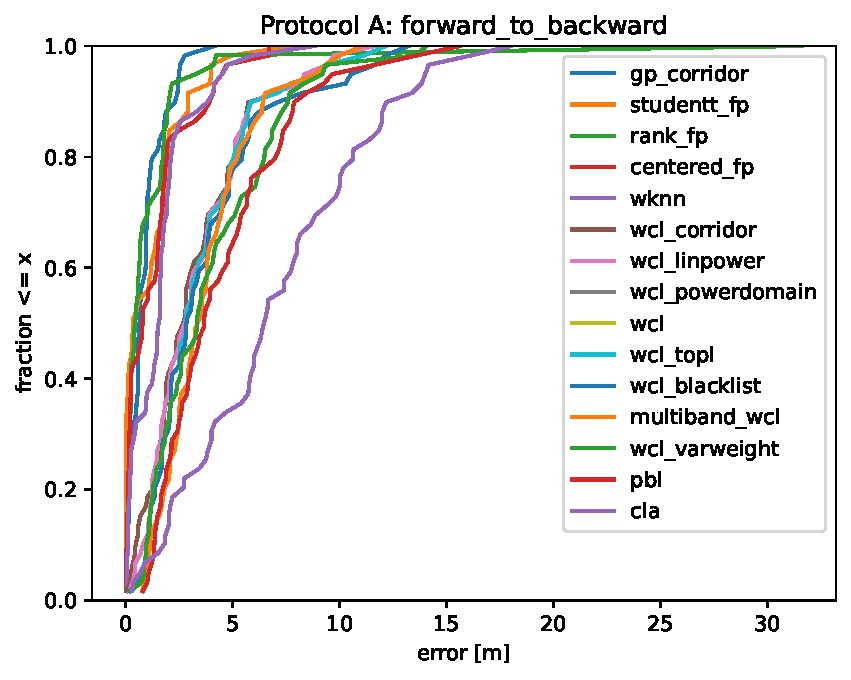
\includegraphics[width=0.5\linewidth]{figures/cdf_protocol_a_forward_to_backward.pdf}\hfill
  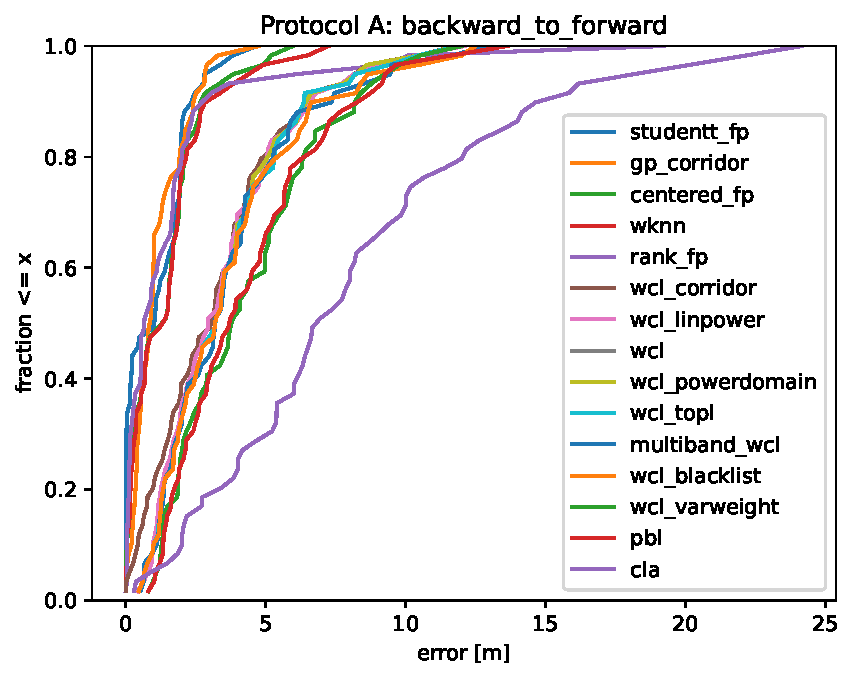
\includegraphics[width=0.5\linewidth]{figures/cdf_protocol_a_backward_to_forward.pdf}
  \caption{Protocol~A 誤差 CDF（左：forward$\to$backward，右：backward$\to$forward）．}
  \label{fig:cdf_pa}
\end{figure*}

\begin{figure*}[t]\centering
  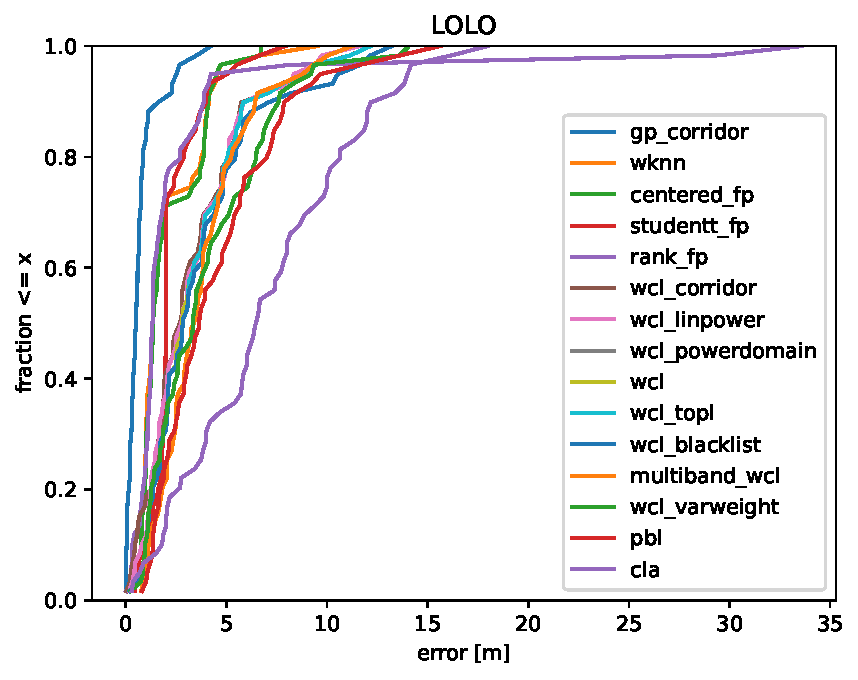
\includegraphics[width=0.40\linewidth]{figures/cdf_lolo.pdf}\hfill
  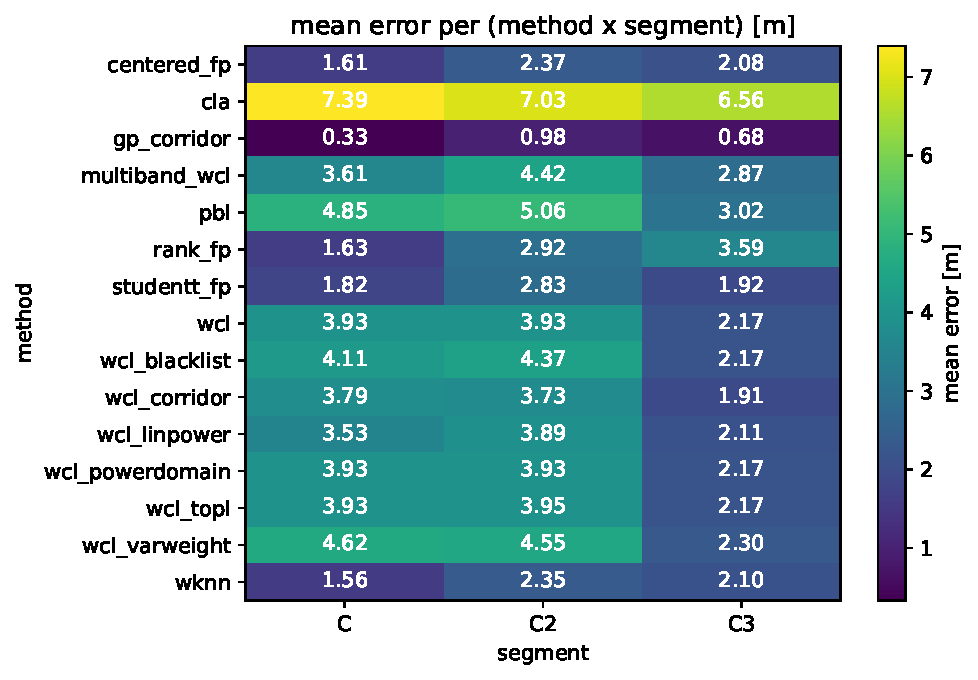
\includegraphics[width=0.58\linewidth]{figures/segment_heatmap.pdf}
  \caption{左：LOLO 誤差 CDF．右：(手法$\times$廊下セグメント) 別の平均誤差 [m]（LOLO ledger）．}
  \label{fig:cdf_lolo_heat}
\end{figure*}

\noindent 要点：
\begin{itemize}
  \item \textbf{gp\_corridor}：LOLO で Ave~0.72~m，中央値~0.50~m，P90~1.74~m，$\leq$2~m 率~90\% と\textbf{目標を達成}．Protocol~A では WCL との差が $-2.61$~m（95\%~CI $[-3.27,-1.94]$，fold~forward$\to$backward）で\textbf{統計的に有意}．
  \item \textbf{Tier~1/2 fingerprinting 系}（LOLO ave）：wknn~2.07 / centered\_fp~2.08 / studentt\_fp~2.32 / rank\_fp~2.70．いずれも WCL~3.51 を大幅に改善．
  \item \textbf{WCL 改良系（Tier~3，LOLO ave）}は小幅：廊下射影~3.31（改善），linpower~3.36（微改善），top-$L$~3.52（同等），blacklist~3.77・varweight~4.04・multiband~3.82（\textbf{悪化}）．凸包制約を保持したままの重み調整では 2~m を切れないことが確認された~\cite{ji2012vap}．
\end{itemize}

\smallskip\noindent\textbf{4.2\; 考察}\;

\noindent\textbf{(a) Protocol~A の位置づけ．}\;
Protocol~A は同一 59 地点を train/test 双方に含むため，測っているのは\textbf{測量済み地点の再認識}であって空間汎化ではない．
実運用で問われる未知地点への一般化を保証するのは LOLO であり，本研究では LOLO を\textbf{決定的テスト}とみなす．Protocol~A の数値は上限性能の目安として補助的に読むべきである．

\noindent\textbf{(b) LOLO $<$ Protocol~A の一見逆転．}\;
gp\_corridor は LOLO（0.72）が Protocol~A の fold 平均（1.01）より\emph{良い}．これは通常と逆であり注意を要する．
仮説として，Protocol~A では同方向の往復差（身体遮蔽・保持方向による方向依存オフセット）に GP が過適合し得るのに対し，LOLO では保持地点を除いた近傍からの平滑補間が結果的に復路クエリへよく整合する，という機構を提示する（\textbf{断定はしない}）．
なお，分割 iterator による構造的除外という既知の経路は，spy テスト（held-out 地点が \texttt{fit} に渡らないことを検証）とコードレビューによる監査で検出されなかった．この逆転をリークで説明する根拠はない．

\noindent\textbf{(c) 負の結果の解釈（仮説，未検証）．}\;
以下はいずれも観測結果に対する\textbf{仮説}であり，対象アブレーションによる検証は未実施である．blacklist の悪化は\textbf{情報源の喪失}という仮説で説明できる：廊下外の AP-C0-3F-04 も位置固有の検出パターンを持ち，除外は識別情報を捨てる．
varweight の悪化は $n{=}10$ の per-query 分散推定がノイジーで重みがかえって不安定になるという仮説による．
multiband の悪化は帯域分割により per-band の有効 AP 数が枯渇し各バンド単体の WCL が劣化するという仮説による．
いずれも確定的な原因特定には的を絞ったアブレーション（例：AP-C0-3F-04 を戻した blacklist の再実行）が必要である．

\noindent\textbf{(d) wcl\_powerdomain $\equiv$ WCL．}\;
重み $w_j=10^{r_j/10}$ は重心の正規化で定数因子が消えるため WCL と\textbf{数学的に同値}である．
実装でも重み正規化は rtol/atol~$1\times10^{-14}$ で一致し，推定座標の差は $<1\times10^{-9}$~m（テスト保証），Protocol~A の delta も浮動小数点精度で 0（$|\Delta|\lesssim10^{-14}$~m）である．
両表とも該当行に短剣符 †（脚注「mathematically $\equiv$ WCL」）を付している．

\noindent\textbf{(e) studentt\_fp の $\beta$ の位置．}\;
中間報告§3.3 の式では $\beta_{a,b}$ が検出項を含む括弧全体に掛かっていたが，実装では $\beta_{a,b}$ を\textbf{RSSI 尤度項のみ}に掛ける形へ意図的に修正した．
検出項は count（Bernoulli）に基づく証拠であり，RSSI の分散に由来する信頼度重みとは単位が異なるため，両者を同一係数で混ぜないための処置である．

\smallskip\noindent\textbf{4.3\; 制約と今後}\;
\begin{itemize}
  \item \textbf{未実装領域}：Tier~4/5（Mahalanobis 距離・PLS 回帰・HMM/Viterbi 等，手法13--21）は本報告では未実装．時系列（順序）情報の利用は「RSSI のみ」の主張と整合させるため慎重を要する．
  \item \textbf{打ち切り観測の代替}：非検出尤度 $P(R<T_b)$ は帯域別しきい値 $T_b$ が復元不能なため，Bernoulli 検出モデルで代替した．
  \item \textbf{追加データ}：C4F 系の追加データ（dataset\_r0701）は本報告では未評価であり，今後の外部妥当性検証の対象とする．
  \item \textbf{データ規模}：59 地点 $\times$ 2 方向という小規模データであり，大規模 ML より説明可能な統計モデルを採ったのは過学習回避のためでもある．結論の一般化には規模拡大が望ましい．
  \item \textbf{実機展開}：先行研究~\cite{tanaka2023tut}と同様のスマートフォン実装（Android アプリ化）への展開は今後の課題である．
\end{itemize}

\section{グループ内で自分が貢献したところ}

\begin{itemize}
  \item ベースライン再現ライブラリ \texttt{icsr8} の設計・実装（仕様書に未記載の暗黙前処理の特定を含む）．
  \item Tier~1--3 の 12 手法および Tier~4 の 7 手法の実装．
  \item 評価ハーネス（Protocol~A・LOLO 分割 iterator，リーク防止 spy テスト，paired bootstrap）の構築．
  \item 検証パイプライン（\texttt{verify\_report.py}・凍結契約テスト）の構築．
  \item 図表の自動生成．
  \item 本報告書および発表スライドの執筆．
\end{itemize}
（グループ内分担の詳細は提出前に調整: [他メンバーの貢献をここに追記]）

\begin{thebibliography}{9}\footnotesize
  \bibitem{tanaka2023tut}
    田中空斗, 足立裕基, 小松和暉, 宮路祐一, 上原秀幸,
    ``大学構内における Wi-Fi の受信信号強度とスマートフォンを用いた屋内位置推定システムの開発,''
    信学論 B, Vol.~J107-B, No.~3, pp.~209--217, Mar.~2024.
    DOI: 10.14923/transcomj.2023GWP0012.
  \bibitem{blumenthal2007wcl}
    J.~Blumenthal, R.~Grossmann, F.~Golatowski, and D.~Timmermann,
    ``Weighted Centroid Localization in Zigbee-Based Sensor Networks,''
    \emph{Proc. IEEE International Symposium on Intelligent Signal Processing (WISP)}, pp.~1--6, Oct.~2007.
    DOI: 10.1109/WISP.2007.4447528.
  \bibitem{bulusu2000gpsless}
    N.~Bulusu, J.~Heidemann, and D.~Estrin,
    ``GPS-Less Low-Cost Outdoor Localization for Very Small Devices,''
    \emph{IEEE Personal Communications}, Vol.~7, Issue~5, pp.~28--34, Oct.~2000.
    DOI: 10.1109/98.878533.
  \bibitem{ji2012vap}
    M.~Ji, Y.~Cho, J.~Kim, Y.~Lee, and S.~Park,
    ``Improving the Positioning Accuracy Using Virtual Access Points in the Border Area,''
    \emph{Proc. International Conference on Indoor Positioning and Indoor Navigation (IPIN 2012)}, Nov.~2012.
  \bibitem{ferris2007gpslam}
    B.~Ferris, D.~Fox, and N.~Lawrence,
    ``WiFi-SLAM Using Gaussian Process Latent Variable Models,''
    \emph{Proc. 20th International Joint Conference on Artificial Intelligence (IJCAI 2007)}, 2007.
  \bibitem{youssef2005horus}
    M.~Youssef and A.~Agrawala,
    ``The Horus WLAN Location Determination System,''
    \emph{Proc. 3rd International Conference on Mobile Systems, Applications, and Services (MobiSys 2005)}, pp.~205--218, 2005.
    DOI: 10.1145/1067170.1067193.
  \bibitem{hara2010statloc}
    原 晋介,
    ``位置推定における統計的推定理論,''
    \emph{IEICE Fundamentals Review}, Vol.~4, No.~1, pp.~32--38, Jul.~2010.
    DOI: 10.1587/essfr.4.32.
  \bibitem{subedi2017}
    S.~Subedi and J.-Y.~Pyun,
    ``Practical Fingerprinting Localization for Indoor Positioning System by Using Beacons,''
    \emph{Journal of Sensors}, Vol.~2017, Article ID 9742170, 16 pages, Dec.~2017.
    DOI: 10.1155/2017/9742170.
  \bibitem{subedi2019}
    S.~Subedi, H.-S.~Gang, N.~Y.~Ko, S.-S.~Hwang, and J.-Y.~Pyun,
    ``Improving Indoor Fingerprinting Positioning With Affinity Propagation Clustering and Weighted Centroid Fingerprint,''
    \emph{IEEE Access}, Vol.~7, pp.~31738--31750, Mar.~2019.
    DOI: 10.1109/ACCESS.2019.2902564.
\end{thebibliography}

\clearpage
\appendix

\section{Tier 4 手法の追補評価}

本付録は本文\textbf{凍結後の追補}であり，本文「制約と今後」で Tier~4/5 を未実装とした記述は\textbf{本付録により更新される}：Tier~4 の 7 手法（手法13--15,17--20）を凍結ベースライン上へ実装・評価した（Tier~5 の時系列手法21 は「RSSI のみ」の主張との整合上，引き続き未実装）．
なお手法16（segment-first）は独立手法ではなく，本文§3.2 の gp\_corridor の\textbf{内部段}（セグメント分類 C/C2/C3 $\to$ セグメント内 1D 推定）として\textbf{実装済み}であり，本付録では単独評価しない（本文の「手法3+16」表記の明確化であって修正ではない）．
評価プロトコル・分割・ブートストラップは本文と\textbf{完全に同一}で，結果は本文成果物と別系統へ隔離してある（CSV は \texttt{results/tier4/}，表・図は既存ディレクトリ内の \texttt{tier4\_*} 固有名：\texttt{tables/tier4\_*.tex}・\texttt{figures/cdf\_lolo\_tier4.pdf}）．

\smallskip\noindent\textbf{A.1\; 手法}\;
7 手法はいずれも地点別 (ap\_name, band) 統計を特徴の基礎とするが，実際に消費する統計は手法ごとに異なる（fisher\_wknn: $\mu/\sigma$；mahalanobis\_wknn: $\mu$＋スキャン残差共分散；pls\_corridor / ordinal\_corridor: $\mu$ のみ；wcl\_residual: $\mu$＋WCL 弧長 $s_{\mathrm{wcl}}$；joint\_fp: $\mu/\sigma/\hat q$；gp\_augmented\_wknn: $\mu/\hat q$）．ハイパーパラメータは train 内 5-fold inner-CV（seed=0，本文 wknn 等と同一契約）で選ぶ．弧長系の pls/ordinal/wcl\_residual/gp\_augmented は train 地点座標を廊下弧長 $s$ への変換に用い，wcl\_residual はさらに WCL 弧長そのものを特徴に含む（AP 座標も使う唯一の手法）；他は AP 座標を使わない純指紋系である．いずれもリーク除外は本文と同一の分割 iterator 契約で保証する．

\smallskip\noindent\textit{fisher\_wknn}（手法13）\;鍵 $k$ ごとに地点間分散/地点内分散の比 Fisher score を計算し，上位 $M$ 鍵に絞った特徴空間で通常の WKNN を行う．分子・分母とも $\sigma$ が有限（検出地点数 $\geq 3$）な地点集合で評価する（母集団の不一致を避ける）．$M\in\{8,16,24,32,48,\text{all}\}$，$k\in\{3,5\}$，weighting $\in\{$inv,inv\_sq$\}$．
\[
  F_k=\frac{\operatorname{Var}_l(\mu_{l,k})}{\operatorname{mean}_l(\sigma_{l,k}^2)}\quad(\sigma\text{ 有限地点のみ}).
\]

\smallskip\noindent\textit{mahalanobis\_wknn}（手法14）\;WKNN の L2 距離を Mahalanobis 距離へ置換する．採択された \texttt{within} モードは，地点等重みの残差外積平均 $\bar S$ に Ledoit--Wolf の\textbf{縮小係数 $\lambda$ のみ}（スキャン残差から算出）を借りて縮小する（生の標本共分散は地点数 $\leq$ 特徴次元で特異なため）．全 fold で \texttt{within} を選択した．
\[
  \bar S=\frac1L\sum_{l}\frac1{n_l}\sum_i(r_i-\mu_l)(r_i-\mu_l)^\top,
\]
\[
  \hat\Sigma=(1-\lambda)\bar S+\lambda\tfrac{\operatorname{tr}\bar S}{p}I,\quad
  d^2=(r-\mu)^\top\hat\Sigma^{-1}(r-\mu).
\]

\smallskip\noindent\textit{pls\_corridor}（手法15）\;標準化した $\mu$ 行列を廊下弧長 $s=\texttt{xy\_to\_arclength}(x,y)$ へ PLS 回帰する（$r\approx TP^\top,\ s\approx Tq$）．廊下が 1 次元多様体であることを用い，高共線な高次元特徴を少数潜在成分に圧縮して 1 スカラー $s$ を予測する．潜在成分数 $\in\{2,3,4,6,8,10\}$．

\smallskip\noindent\textit{ordinal\_corridor}（手法17）\;train 弧長 $s$ の分位点を閾値 $c_1<\dots<c_m$（水準 $k/(m{+}1)$）とし，各閾値で二値ロジット $P(s>c_k\mid r)=\sigma(f_k(z))$ を独立 fit，isotonic 回帰で非増加へ射影後，生存関数の階段積分で期待弧長を再構成する．$m\in\{8,12\}$，$C\in\{0.1,1,10\}$．
\[
  \hat s=s_{\min}+\sum_{k=0}^{m}p_k\,(c_{k+1}-c_k),
\]
\[
  p_0:=1,\quad c_0:=s_{\min},\quad c_{m+1}:=s_{\max}.
\]

\smallskip\noindent\textit{wcl\_residual}（手法18）\;baseline WCL の弧長推定 $s_{\mathrm{wcl}}$ を，$[$標準化 $\mu$ 行列$,\ s_{\mathrm{wcl}}]$ を特徴とする Ridge 回帰の残差 $g(\cdot)$ で補正する：$\hat s=\operatorname{clip}(s_{\mathrm{wcl}}+g(\cdot))$，目標は $s_{\text{true}}-s_{\mathrm{wcl}}$（WCL が説明できない誤差のみを学習）．$\alpha\in\{0.1,1,10,100\}$．
なお WC 出力を指紋特徴量へ統合する発想は BLE 屋内測位に先行例がある \cite{subedi2017,subedi2019}．

\smallskip\noindent\textit{joint\_fp}（手法19）\;RSSI 残差項に検出率の複合項を足した距離を用いる．検出率は $\hat d=(n_{\text{detect}}{+}1)/(n_{\text{scan}}{+}2)$（Beta$(1,1)$ 平滑化）．\textbf{全 train 鍵}で和を取り，未検出 $r/\mu$ は NON\_DETECT，未適格 $\sigma$ は SIGMA\_MIN で埋める（共通検出鍵のみに絞る旧実装は遠方地点の偶然一致で破綻したため）．$\eta\in\{0,0.5,1,2,4\}$，$k\in\{3,5\}$．
\[
  d(q,l)=\frac1{|K|}\sum_{k\in K}\frac{(r_k-\mu_{l,k})^2}{\sigma_{l,k}^2+\varepsilon}
         +\frac{\eta}{|K|}\sum_{k\in K}(\hat d_k-\hat q_{l,k})^2.
\]

\smallskip\noindent\textit{gp\_augmented\_wknn}（手法20）\;各鍵の RSSI を弧長 $s$ の 1D GP でモデル化し（gp\_corridor の GP 部品を再利用），間隔 $\Delta$ の $s$ グリッド上に仮想参照点 $\mu_k(s)$ を合成する．検出率 $\hat q(s)<0.5$ の領域は NON\_DETECT へゲートし（検出フットプリント外の外挿を抑止），実測点＋仮想点の合同集合へ WKNN，仮想点の重みを $w_{\text{virt}}$ で減衰する．inner-CV は $(\Delta,w_{\text{virt}},k)$ のみを順位付けする前処理なので\textbf{縮小 GP グリッド}（単一中スケール config）で安価に回し，最終 radio map のみ全グリッドで fit する．$\Delta\in\{2,4\}$，$w_{\text{virt}}\in\{0.25,0.5,1\}$，$k\in\{5,7\}$．

\smallskip\noindent\textbf{A.2\; 実験}\;
本文と\textbf{同一}のプロトコル（Protocol~A 2 fold ＋ LOLO 59 fold，分割 iterator による構造的リーク除外の spy 契約，地点別誤差上の paired bootstrap $B{=}1000$, seed=0，95\% CI）で 7 手法＋参照 2 手法（wcl, gp\_corridor）を評価した．
\textbf{主要比較は各手法 vs gp\_corridor（本文で目標を達成した手法）を事前指定}し，vs WCL を含むその他は\textbf{探索的}とする．多重比較補正は行わず，探索的比較として読む（A.5）．

\smallskip\noindent\textbf{A.3\; 結果}\;
Protocol~A を表\ref{tab:tier4_pa}，LOLO を表\ref{tab:tier4_lolo}，LOLO 誤差 CDF を図\ref{fig:tier4_cdf}に示す（数値は表生成器の \%.2f 出力を直接 \texttt{\textbackslash input}）．

\begin{table*}[t]\centering\footnotesize
\setlength{\tabcolsep}{3.2pt}
\caption{Tier~4：Protocol~A（両方向 2 fold）の手法別誤差 [m]．$\Delta$wcl / $\Delta$gp\_corridor は各参照との差（負ほど良い）．行は LOLO ave 昇順．$^{\ast}$ は主要比較基準 gp\_corridor．}
\label{tab:tier4_pa}
\begin{tabular}{llrrrrrrrr}
\toprule
Method & Fold & Ave & Median & P90 & Within 2m & Max & Std & $\Delta$wcl & $\Delta$gp\_corridor \\
\midrule
gp\_corridor$^{\ast}$ & backward\_to\_forward & 1.12 & 0.89 & 2.44 & 0.81 & 4.76 & 0.96 & -2.45 & 0.00 \\
gp\_corridor$^{\ast}$ & forward\_to\_backward & 0.90 & 0.66 & 2.32 & 0.88 & 4.17 & 0.84 & -2.61 & 0.00 \\
mahalanobis\_wknn & backward\_to\_forward & 1.14 & 0.95 & 2.03 & 0.86 & 4.60 & 0.97 & -2.43 & 0.02 \\
mahalanobis\_wknn & forward\_to\_backward & 1.06 & 0.49 & 2.63 & 0.81 & 4.75 & 1.15 & -2.45 & 0.16 \\
gp\_augmented\_wknn & backward\_to\_forward & 1.49 & 1.02 & 3.56 & 0.69 & 6.04 & 1.34 & -2.08 & 0.37 \\
gp\_augmented\_wknn & forward\_to\_backward & 1.44 & 1.33 & 3.02 & 0.75 & 5.39 & 1.18 & -2.08 & 0.54 \\
joint\_fp & backward\_to\_forward & 1.82 & 1.51 & 4.09 & 0.66 & 7.40 & 1.71 & -1.75 & 0.71 \\
joint\_fp & forward\_to\_backward & 1.58 & 1.13 & 3.16 & 0.76 & 9.09 & 1.68 & -1.93 & 0.68 \\
fisher\_wknn & backward\_to\_forward & 1.37 & 1.44 & 2.60 & 0.76 & 6.51 & 1.34 & -2.20 & 0.25 \\
fisher\_wknn & forward\_to\_backward & 1.75 & 1.25 & 3.83 & 0.76 & 11.21 & 2.11 & -1.76 & 0.85 \\
wcl\_residual & backward\_to\_forward & 2.68 & 2.30 & 5.54 & 0.44 & 8.54 & 1.93 & -0.89 & 1.56 \\
wcl\_residual & forward\_to\_backward & 2.87 & 2.09 & 5.76 & 0.47 & 10.24 & 2.30 & -0.64 & 1.97 \\
wcl & backward\_to\_forward & 3.57 & 3.22 & 6.48 & 0.32 & 11.85 & 2.42 & 0.00 & 2.45 \\
wcl & forward\_to\_backward & 3.51 & 2.81 & 6.09 & 0.31 & 12.17 & 2.54 & 0.00 & 2.61 \\
pls\_corridor & backward\_to\_forward & 3.44 & 2.55 & 7.43 & 0.36 & 12.49 & 2.78 & -0.13 & 2.32 \\
pls\_corridor & forward\_to\_backward & 3.49 & 3.04 & 6.98 & 0.34 & 10.24 & 2.52 & -0.03 & 2.59 \\
ordinal\_corridor & backward\_to\_forward & 5.14 & 4.81 & 9.10 & 0.10 & 10.00 & 2.57 & 1.57 & 4.02 \\
ordinal\_corridor & forward\_to\_backward & 4.16 & 4.02 & 6.70 & 0.19 & 9.55 & 2.23 & 0.65 & 3.26 \\
\bottomrule
\end{tabular}
\par\footnotesize $^{\ast}$ gp\_corridor: 主要比較基準。

\end{table*}

\begin{table}[t]\centering\footnotesize
\resizebox{\linewidth}{!}{
\begin{tabular}{lrrrrrr}
\toprule
Method & Ave & Median & P90 & Within 2m & $\Delta$wcl & $\Delta$gp\_corridor \\
\midrule
gp\_corridor$^{\ast}$ & 0.72 & 0.50 & 1.74 & 0.90 & -2.79 & 0.00 \\
mahalanobis\_wknn & 1.77 & 1.29 & 3.82 & 0.76 & -1.75 & 1.04 \\
gp\_augmented\_wknn & 1.87 & 1.70 & 3.66 & 0.58 & -1.64 & 1.15 \\
joint\_fp & 2.09 & 1.40 & 4.19 & 0.61 & -1.42 & 1.37 \\
fisher\_wknn & 2.12 & 1.50 & 4.25 & 0.66 & -1.39 & 1.40 \\
wcl\_residual & 3.24 & 2.46 & 6.23 & 0.41 & -0.27 & 2.52 \\
wcl & 3.51 & 2.81 & 6.09 & 0.31 & 0.00 & 2.79 \\
pls\_corridor & 3.79 & 3.21 & 8.35 & 0.39 & 0.28 & 3.07 \\
ordinal\_corridor & 4.60 & 4.46 & 7.45 & 0.17 & 1.09 & 3.88 \\
\bottomrule
\end{tabular}
\par\footnotesize $^{\ast}$ gp\_corridor: 主要比較基準。

}
\caption{Tier~4：LOLO（59 fold）の手法別誤差 [m] と参照との差．空間+方向汎化の決定的テスト．行は ave 昇順．}
\label{tab:tier4_lolo}
\end{table}

\begin{figure}[t]\centering
  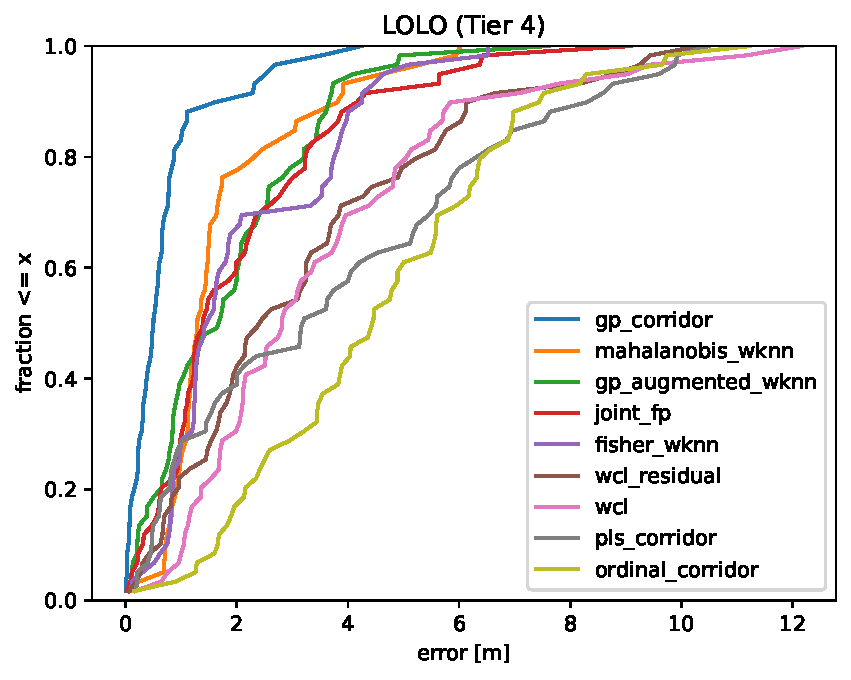
\includegraphics[width=0.9\linewidth]{figures/cdf_lolo_tier4.pdf}
  \caption{Tier~4：9 手法（7 Tier4 ＋ 参照 wcl/gp\_corridor）の LOLO 誤差 CDF．}
  \label{fig:tier4_cdf}
\end{figure}

\smallskip\noindent\textbf{A.4\; 考察}\;
\textbf{主要比較（vs gp\_corridor）では 7 手法すべてが有意に劣る}：LOLO の $\Delta$gp\_corridor はいずれも 95\% CI 下限が正で（mahalanobis~$1.04$ $[0.69,1.38]$ / gp\_augmented~$1.15$ $[0.83,1.47]$ / joint\_fp~$1.37$ $[0.95,1.79]$ / fisher~$1.40$ $[0.98,1.80]$，以下 wcl\_residual~$2.52$・pls~$3.07$・ordinal~$3.88$），gp\_corridor 超えは達成できなかった．
一方 \textbf{WKNN 系 4 手法は vs WCL で有意改善}し 2~m 前後に収まる：mahalanobis~$1.77$（$\Delta$wcl $-1.75$~m，95\%~CI $[-2.49,-1.01]$）/ gp\_augmented~$1.87$（$-1.64$，$[-2.39,-0.84]$）/ joint\_fp~$2.09$（$-1.42$，$[-2.18,-0.61]$）/ fisher~$2.12$（$-1.39$，$[-2.09,-0.65]$）．
\textbf{wcl\_residual}（$\Delta$wcl $-0.27$，$[-1.07,0.52]$）と \textbf{pls}（$0.28$，$[-0.65,1.19]$）は WCL と\textbf{有意差なし}，\textbf{ordinal}（$1.09$，$[0.26,1.88]$）は\textbf{有意に悪化}した．
悪化・非有意の機構は以下の\textbf{仮説（未検証）}である：ordinal は 59 標本（inner-CV fold ではさらに少数）で閾値ごとの二値ロジットが不安定になり分位点閾値の識別が揺れる；pls は高共線・小標本で位置関連の潜在成分方向が定まりにくい；wcl\_residual は WCL の凸包バイアスを弧長残差だけでは吸収しきれない．いずれも確定には的を絞ったアブレーションを要する．

\smallskip\noindent\textbf{A.5\; Limitations}\;
\begin{itemize}
  \item \textbf{fisher の MI 項省略}：mRMR の相互情報量項は，59 地点では MI 推定の分散が過大で選択をかえって不安定化するため省き，単変量 Fisher 比のみで鍵選択した．
  \item \textbf{手法20 の GP 利用範囲}：仮想点には GP 事後\textbf{平均のみ}を用い，事後分散からのサンプリング（$\tilde r_a(s)\sim\mathcal N(\mu_a(s),v_a(s)+\sigma^2)$）は不採用．
  \item \textbf{joint\_fp の $\eta$ 境界解}：Protocol~A では両 fold ともグリッド上限 $\eta{=}4.0$ を選択する境界解であり，検出項 $(\hat d-\hat q)^2$ の寄与が RSSI 項に比して弱いことを示唆する（LOLO では fold により $\eta\in\{0,2,4\}$ が混在）．
  \item \textbf{記述的 CI}：地点 bootstrap は地点間の空間相関を無視した地点独立仮定下の\textbf{記述的 CI}である．
  \item \textbf{多重比較}：主要比較以外は探索的で多重比較補正を行っておらず，有意性は探索的に解釈すべきである．
\end{itemize}

\section{再現手順}

\begin{enumerate}
  \item \texttt{uv sync} で依存を解決．
  \item \texttt{uv run pytest}（364 テスト）が全て通ることを確認．
  \item \texttt{uv run python scripts/run\_all\_methods.py --methods}〈本文 15 手法名〉で CSV・図・TeX 断片を再生成（\texttt{--methods} を省略すると登録済み Tier~4 手法まで掃引し本文成果物を上書きするため不可．Tier~4 は \texttt{scripts/run\_tier4.py} で別系統に再生成）．
  \item \texttt{uv run python scripts/dump\_method\_diagnostics.py} で \texttt{results/method\_diagnostics.csv}（\S3 引用値の根拠）を再生成．
  \item \texttt{(cd doc/final\_report \&\& latexmk -lualatex main.tex)} で本 PDF をビルド．
  \item リポジトリルートで \texttt{uv run python scripts/verify\_report.py} を実行し，表数値・診断値・参照パスの整合を検証．
\end{enumerate}

\end{document}
